\documentclass[conference]{IEEEtran}
\usepackage{cite}
\usepackage{graphicx}
\usepackage{multirow}
\usepackage{amssymb}
\usepackage{siunitx}
\usepackage{dcolumn}

% correct bad hyphenation here
\hyphenation{op-tical net-works semi-conduc-tor}


\newcommand{\toolName}{OUR TOOL}

\begin{document}
%
% paper title
% Titles are generally capitalized except for words such as a, an, and, as,
% at, but, by, for, in, nor, of, on, or, the, to and up, which are usually
% not capitalized unless they are the first or last word of the title.
% Linebreaks \\ can be used within to get better formatting as desired.
% Do not put math or special symbols in the title.
\title{\toolName: Navigating Program Flow in the IDE}


% author names and affiliations
% use a multiple column layout for up to three different
% affiliations
\author{\IEEEauthorblockN{Chris Brown, Justin Smith, Tyler Albert, and Emerson Murphy-Hill}
\IEEEauthorblockA{Department of Computer Science\\
North Carolina State University\\
Raleigh, North Carolina 27606\\
Email: \{dcbrow10, jssmit11, tralber2\}@ncsu.edu, emerson@csc.ncsu.edu}
}

% make the title area
\maketitle

% As a general rule, do not put math, special symbols or citations
% in the abstract
\begin{abstract}
Program navigation is a critical task for software developers. 
Unfortunately, the current state-of-the-art tools do not adequately support developers in simultaneously navigating both control flow and data flow (i.e. program flow). 
To assist developers in effectively navigating program flow we designed and implemented a tool that leverages powerful program analysis techniques while maintaining low barriers to invocation.
Our tool enables developers to systematically navigate program flow upstream and downstream within the Eclipse Integrated Development Environment (IDE).
Based on a preliminary evaluation with 8 programmers, our tool compares well to existing tools. 
%Something about tradeoffs.
%For simple sub-tasks tool was effective with very few interface elements. 
\end{abstract}

% no keywords



\IEEEpeerreviewmaketitle


\section{Introduction}
%Probably need to add in the minimalist angle. How much can we achieve with minimal alterations to the IDE.
%Existing tools feature many cumbersome UI widgets or seem poorly integrated into the IDE.
%
Modern software systems contain millions of lines of source code. 
As software grows in size and complexity, developers increasingly rely on tools to help them navigate the programs they create. 
Program navigation is a central task tied to many critical activities, including exploring new code bases, debugging, and assessing security vulnerabilities. 

While navigating programs, developers ask questions about control flow and data flow throughout the program~\cite{latoza2010hard, Smith2015}. We will refer to these two concepts together as \textit{program flow}. Developers are interested in navigating program flow to trace how data is modified across multiple method invocations.

Integrated development environments (IDEs) present code linearly in the order methods are defined. However, successful developers do not navigate source code linearly (line by line starting at the top of the file). Instead, they methodically navigate the code's hierarchical semantic structures~\cite{robillard2004investigate}. To resolve this conflict and realize their ideal navigation strategies, developers rely on program navigation tools. 

% Much work has focused on helping developers visualize and navigate call graphs,
% we also interested in 
% Probably more to come in here? What are some current tools and why are they limited.
% Discuss program visualization tools vs navigation tools.

In this work we designed, implemented, and evaluated a program navigation tool.
To address the limitations of existing program navigation tools, \toolName embodies four key design principles (Section \ref{DesignPrinciples}).

%This paper makes the following contributions:


\section{Design Principles}
\label{DesignPrinciples}
In this section we describe the design principles that we used to shape \toolName. We derived these design principles by examining existing program navigation tools.
 
\vspace{1em} 
\noindent\textbf{Powerful Program Analysis} ---
Simple textual analysis may lead to inaccurate results in many scenarios. For example, such analysis fails when programs include duplicated variable names that refer different variables in different scopes. Textual analysis also falls short when programs contain inheritance and when variable names are included in comments, doccumentation, or other syntactically irrelevant locations.
By leveraging powerful program analysis techniques, navigation tools can provide more accurate information than simple textual analysis.
By analyzing abstract syntax trees (ASTs) and call graphs, tools can make proper references to variables and methods. 

\vspace{1em} 
\noindent\textbf{Low Barriers to Invocation} ---
Barriers to invocation may inhibit adoption. 
As developers may wish to navigate multiple program paths concurrently, repetitively invoking the tool may be cumbersome, especially if barriers are high. 


\vspace{1em} 
\noindent\textbf{Full Program Navigation}  ---
Developers are not only interested in traversing programs' call graphs, but also how data flows through the call graph.
To do so, developers must inspect the relationship between methods as well as the methods themselves.
Often the methods of interest span across multiple source files.
Furthermore, program navigation tools should support this traversal both upstream and downstream. 
That is, tools should highlight variable assignments and also subsequent variable uses. 

\vspace{1em} 
\noindent\textbf{In Situ Navigation}  ---
Switching between views in the IDE can cause disorientation~\cite{deAlwis2006disorient}. As developers navigate through code, navigation tools should present their results in that context. 
When navigation tools present results outside the code, developers are burdened with the cognitive load of translating those results back to the code.

\section{Background}
%Summary of related work, including a table evaluating existing %tools on various design principles.
%Spoiler alert, none of the tools satisfy all of the principles.
There are a variety of tools available to help developers explore and navigate code. Here we discuss two types of tools, production tools and visualization tools and Table \ref{table:background} shows a comparison between \toolName~ and other related tools in terms of the four design principles used to implement our tool.

\subsection{Production Tools}
Production tools are represented by plugins in integrated development environments that provide detailed information and analysis on variables and methods in the source code. Examples of these types of tools include \emph{Call Hierarchy} and \emph{Find References} in Eclipse\cite{Eclipse} and \emph{Analyze Data Flow To/From Here} and \emph{Analyze Dependencies} in IntelliJ\cite{IntelliJ}. These tools provide powerful program analysis for users to navigate throughout the entirety of a project, however they generally differ from our tool in that they may require multiple steps to start the tool or modify the user's navigation (i.e. switching between up and down search), may need repeated invocations of the plugin to track multiple paths or variables in the code, and force users to switch between the text editor of the IDE and a new panel displaying the results.

There are also several production tools that are strictly consolidated within the editor. Two examples of these types of commercial tools include \emph{Mark Occurrences}\cite{MarkOccurrences} and \emph{Open Declaration} in the Eclipse IDE. These approaches are similar to our tool in that they display the results within the editor rather than a separate view or panel, but in some cases they may not provide a detailed enough analysis to explore the entire program or provide extra unnecessary information, for example Mark Occurrences only highlighting the instances of data within a class in addition to highlighting the value in a comment. These can require repeated work to start the tool, such as Open Declaration requiring the user to right-click or enter a keyboard shortcut for each method or variable declaration the user wants to open.

\subsection{Visualization Tools}
Code navigation tools that provide users with a graphical representation of the results are visualization tools. Some examples of these types of tools include \emph{Code Bubbles}\cite{CodeBubbles}, \emph{Code Canvas}\cite{CodeCanvas}, \emph{Code Surfer}\cite{CodeSurfer}, \emph{Dora}\cite{Dora}, \emph{Reacher}\cite{Reacher}, \emph{Relo}\cite{Relo}, \emph{Whyline}\cite{Whyline}, and many more research tools. These works provide various views of control flow graphs, class and UML-like diagrams, trees, call graphs, and other images to describe the hierarchy and relationship between different variables or functions within the code. \toolName~differs because, while all visualization tools can provide powerful data analysis, but we desire minimal steps to invoke the tool and present the information inside of the editor.

\begin{table}
	\centering
	\caption{Design Principles}
	\begin{tabular}{|c|c|c|c|c|}
		%\rowcolor{gray!50}
		\hline
		Tool & Powerful & Low & Full Prog. & In Situ\\
		%\rowcolor{gray!50}
		 & Analysis & Barriers & Nav. & Nav.\\
		\hline
		Call Hierarchy & \checkmark & - & \checkmark & -\\
		\hline
		Find References & \checkmark & - & \checkmark & -\\
		\hline
		Analyze Data Flow & \checkmark & - & \checkmark & -\\
		\hline
		Analyze Dependencies & \checkmark & - & \checkmark & -\\
		\hline
		Mark Occurrences & - & \checkmark & - & \checkmark \\
		\hline
		Open Declaration & \checkmark & - & \checkmark & \checkmark \\
		\hline
		Code Bubbles & \checkmark & - & \checkmark & \checkmark \\
		\hline
		Code Canvas & \checkmark & - & \checkmark & \checkmark \\
		\hline
		Code Surfer & \checkmark & - & \checkmark & Sometimes \\
		\hline
		Dora & \checkmark & - & \checkmark & - \\
		\hline
		Reacher & \checkmark & - & \checkmark & - \\
		\hline
		Relo & \checkmark & - & \checkmark & - \\
		\hline
		Whyline & \checkmark & - & \checkmark & - \\
		\hline
	\end{tabular}
	\label{table:background}
\end{table}


\section{\toolName}
\toolName~was designed to realize all of the principles described in Section \ref{DesignPrinciples}. 
We implemented \toolName~as a plugin to the Eclipse IDE~\cite{Eclipse}. 
We chose Eclipse because of its popularity and extensibility. 
Eclipse is one of the most widely used open source IDEs for Java development and it provides many extension points for plugins. 

Figure \ref{fig:tool} depicts \toolName~invoked on a variable participants were asked to inspect as part of our evaluation. To visualize how a programmer would interact with \toolName, consider the following scenario:

You are concerned that users could modify the value of \texttt{fileName} before it gets passed into \texttt{getQueries}. 
First, you click on \texttt{fileName} (A). 
To help you locate where the variable is modified and referenced, \toolName~ highlights proper occurrences of that variable in the code.
Since \texttt{fileName} is a formal parameter to \texttt{getQueries}, any method calling \texttt{getQueries} could modify \texttt{fileName}. 
Those methods reside in other class files, so \toolName~ provides links to their locations (B1).
Rather than move your mouse up to the top of the editor window, you click on \texttt{getQueries} (B2), which conveniently links to the first call site, \texttt{createTables}. 
\toolName~ opens \texttt{createTables} and highlights the location in that method where fileName is passed to \texttt{getQueries}.  Additionally, if the selected variable has uses that do not appear in the user's current view of the editor then the tool will provide links to those off-screen line numbers in the top box if it appears above the current location and in the bottom box if it is used below (not shown).

%Something about using \toolName for down flow.
%(A) - When a user clicks on a variable all (visible) instances of that variable are highlighted in the code. (B) - When the variable has been declared as a parameter to the current method, users can click on that method's name in the editor to navigate to a location where that method is called. (X) - When the variable is passed to an external method, users can click on that method's name to open its declaration. (C) - If the variable is passed in from another method or is defined earlier in the current file, a link to that location is displayed in the ``top box.'' (D) - If the variable is passed in to another method or referenced later in the current file, links to those locations appear in the ``bottom box.''

\begin{figure*}
	\centering
	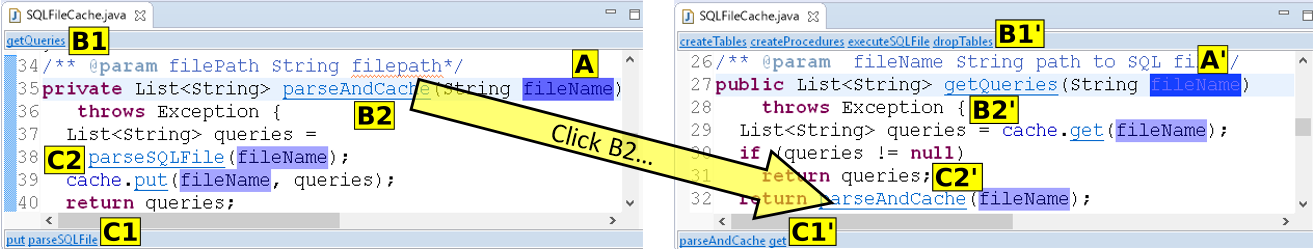
\includegraphics[width=0.75\textwidth]{images/toolScreenshot}
	\caption{Code view in the Eclipse IDE with \toolName~invoked on Task 1}	
	\label{fig:tool} 
\end{figure*}

%TODO- Update image and description for B/C 1/2

\begin{table}
\centering
\caption{Participant Demographics}
\begin{tabular}{|c|S|S|c|}
%\rowcolor{gray!50}
\hline
Participant & \multicolumn{1}{c|}{Industry} & \multicolumn{1}{c|}{Java} &\multicolumn{1}{c|}{Previous} \\
%\rowcolor{gray!50}
& \multicolumn{1}{c|}{Experience (years)} & \multicolumn{1}{c|}{Experience (years)} & \multicolumn{1}{c|}{Eclipse Use} \\
\hline
P1 & 9 & 5 & \checkmark \\
\hline
P2 & 0 & 6 & \checkmark \\
\hline
P3 & 3 & 2 & - \\
\hline
P4 & 5 & 0 & - \\
\hline
P5 & 12 & 10 & \checkmark \\
\hline
P6 & 0 & 3.5 & \checkmark \\
\hline
P7 & 1 & 9 & \checkmark\\
\hline
P8 & 5.5 & 3.5 & \checkmark\\
\hline
\end{tabular}
\label{table:participants}
\end{table}

\section{Preliminary Evaluation}
We performed a preliminary evaluation of \toolName~ with eight programmers performing two code navigation tasks.
Our goals in this study were to get feedback on the usability of our tool and evaluate whether our approach shows promise in enabling developers to effectively navigate program flow. 

All participants were graduate students at the time of the study with a mean of 5 years of professional programming experience; Table \ref{table:participants} provides additional information about each participant. We recruited participants using a convenience sampling approach. 

Each participant used \toolName~for one task and Eclipse's tools (call hierarchy, mark occurrences, and open declaration) for the second task.
To control for learning and fatigue effects, we used a 2x2 latin square design which permuted the order participants received each tool and performed each task. Accordingly, each participant was assigned to one of four groups -- one group for each pair of conditions.
Before the study, we asked participants to report whether they were familiar with the Eclipse IDE. We used this information to balance Eclipse novices across groups.


\subsection{Tasks}
We analyzed the data from our previous study~\cite{Smith2015}, which included two tasks that required program flow navigation.
In the previous study, developers expressed a willingness to navigate the program, but used sub-optimal strategies to do so.
Because the challenges participants faced in ~\cite{Smith2015} partially inspired the development of \toolName, we include the same two tasks in this study.

The two tasks we chose are complementary in that Task 1 required participants to navigate up the call graph, inspecting the callers of the initial method. 
On the other hand, Task 2 required participants to inspect the methods called by the initial method.
For Task 1 we asked participants to tell us whether a method ever receives user-provided input.
For Task 2 we asked participants to tell us whether a form field is validated before being sent to the database.
To ensure all participants had a baseline familiarity with both tools, we trained participants on the appropriate tools preceding each task. 
To evaluate the effectiveness of the navigation tools rather than participants' familiarity with a particular code base, we asked participants to navigate code they had not previously contributed to. 
Because think aloud protocols distort the amount of time required to complete tasks, we did not interrupt or prompt participants until after they had completed the tasks.

%We chose two tasks that (differentiate between the two tasks... up and down?)

\subsection{Usability Evaluation}
To evaluate the usability of \toolName, we administered an adapted version of the Post-Study System Usability Questionnaire (PSSUQ)~\cite{Lewis95ibmcomputer} after participants had completed both tasks. We modified the questionnaire by replacing ``this system'' with ``this tool'' and asked questions from the System Quality and Interface Quality categories. We asked 10 questions; participants responded on a 7-point Likert scale from ``Strongly Disagree'' to ``Strongly Agree.'' 	
To prompt discussion about the usability of \toolName, we also asked participants open-ended questions based on applicable categories from Nielsen's usability heuristics~\cite{Nielsen1992}.
To capture participant's experiences that these two metrics overlooked, two of the authors independently examined each audio/video recording and recorded memos. 

\section{Results}
\subsection{Quant stuff...}
\begin{figure}
	\centering
	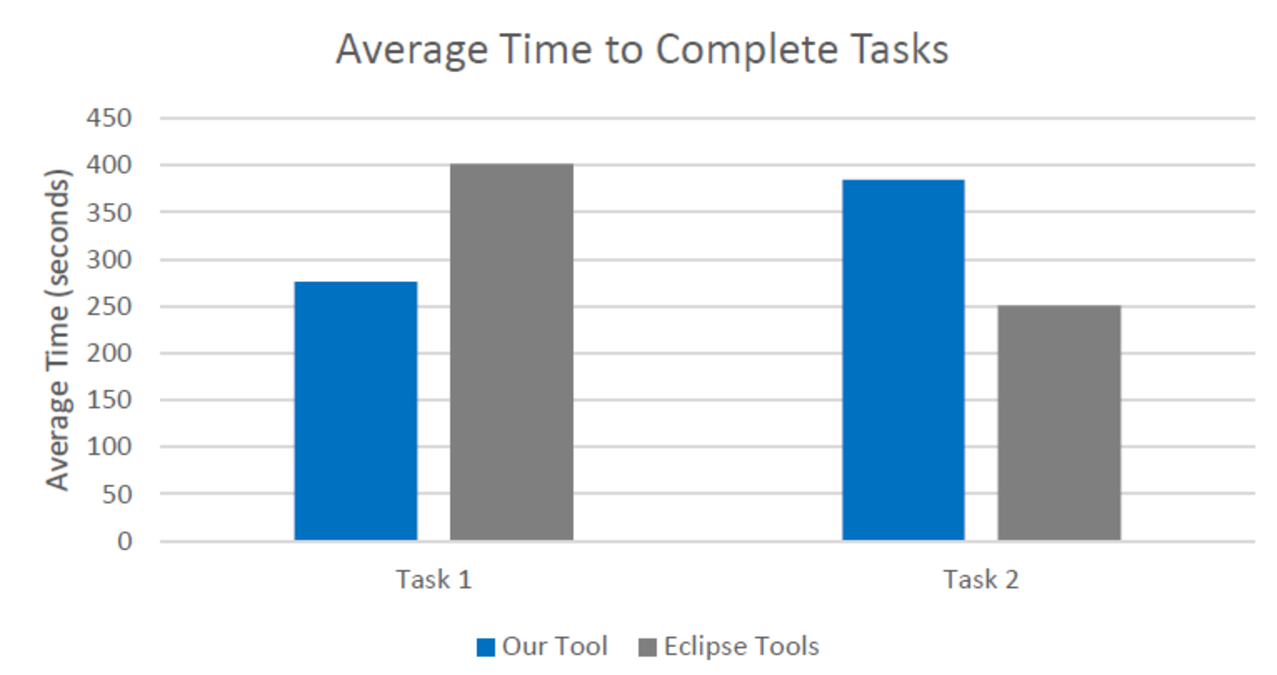
\includegraphics[width=\columnwidth]{images/taskTime}
	\caption{Mean time to complete each task with and without \toolName}
	\label{fig:taskTime} 
\end{figure}


Compared to the Eclipse tools, results with \toolName~ were mixed.
%Overall, task competion time distorts the actual time participants took to complete the task.
%Participants who explored more of the call graph are penalized. 
%Some participants spent additional time exploring after finding the right answer to confirm their conclusion
For Task 1, participants were X\% faster with \toolName~ than the Eclipse tools (Figure \ref{fig:taskTime}). 
(Not sure how to report correctness here... 4 gave the correct answer with eclipse tools --
2 were correct with ours. However, the incorrect two navigated correctly, located a hard-coded parameter, responded incorrectly, and did not justify)
However, participants were Y\% slower for Task 2.
(Correctness in terms of navigation was even split. One with our tool guessed correctly)

To understand why participants were faster for Task 1 with \toolName, we analyzed how long it took participants to navigate one step up the call graph. Participants equipped with our tool were strictly faster than participants with the Eclipse tools with averages of 8 seconds and 44 seconds, respectively. 

On the PSSUQ, participants responded most positively to questions about \toolName's simplicity, how easy it was to use, and how easy it was to learn. 
Median responses to these three questions was 6.
On the other hand, participants responded most negatively to questions about whether the tool provided all the expected functions and capabilities and whether it would enable them to complete tasks quickly.
To these two questions, participants' median response was 5. 
On average, participants who used \toolName~ for Task 1 rated it more highly than those who used the tool for Task 2.


\subsection{Qualitative Results}

After navigating through several chains of method invocations with \toolName, some participants felt like they had reached ``dead ends'' and were unsure of how to navigate back to where they came from. After reaching a top-level method, P1 asked, ``How can I return back to where I came from?'' While working with \toolName~ P6 utilized Eclipse's back buttons to retrace his steps, but still could not reorient himself. 

%All the functions I expected (Missing tracability and mark bars, ... )



\section{Discussion - Scenarios}
List scenarios when our tool worked and when it didn't
\subsection{Wins}
Getting started. Low barriers to invocation
\\
\textbf{Linear Naviagtion}
When participants navigated linearly in one direction (as in Task 1). Our tool was most effective. 
Few branches



\subsection{Losses}
Why were they slower and less accurate with our tool?
Second task: 
Lots of confounding variables meant participants spent time switching between variables.
Requires more knowledge about iTrust. Even though we signposted all the areas that (required) knowledge about iTrust...

Using our tool for task 1, everyone located a hard-coded string. But the two participants that answered incorrectly (misinterreted the information)



\subsection{Systematic Evaluation}
Program navigation tools should help developers keep track of where they have been and where they are going. Especially while attempting to resolve complex defects, developers may want to thoroughly explore all program paths. Their navigation tools should help them keep track of their progress.

\subsection{Design Implications}

Participants were taken to new locations but couldn't backtrack.
	Back buttons exist, but most didn't use and they didn't help the person who did use them...
	Points to an inherent limitation of our minimalistic approach. People would be more oriented with a graph or more persistent breadcrumbs...\\
	Especially important when participants reach ``dead ends.'' When we detect that, intervene!
	
Overwhelmed when the call graph had a high branching factor.
	Participants quickly navigated up single paths as in Task 1
	When call paths branched in many directions our tool could reccomend more full featured tools.\\
Couldn't keep track of where they had been.
	See systematic evaluation. Links could turn purple and get moved to the end of the list.\\
Performance.
	Whenever the user clicks on a new variable \toolName~ has to search through the entire project for locations where the method is declared or invoked. We observed that participants navigated within one file more often than between files. To improve the performance of our tool, we could optimize the search to return local results before returning global search results.	Participants also repeated invocation on the same variables (we could do some caching)


\section{Limitations}

\section{Conclusion}

\section*{Acknowledgment}

The authors would like to thank...





% trigger a \newpage just before the given reference
% number - used to balance the columns on the last page
% adjust value as needed - may need to be readjusted if
% the document is modified later
%\IEEEtriggeratref{8}
% The "triggered" command can be changed if desired:
%\IEEEtriggercmd{\enlargethispage{-5in}}

% references section

% can use a bibliography generated by BibTeX as a .bbl file
% BibTeX documentation can be easily obtained at:
% http://mirror.ctan.org/biblio/bibtex/contrib/doc/
% The IEEEtran BibTeX style support page is at:
% http://www.michaelshell.org/tex/ieeetran/bibtex/
\bibliographystyle{IEEEtran}
% argument is your BibTeX string definitions and bibliography database(s)
\bibliography{progNavPaper}




% that's all folks
\end{document}
